\section{Linear Factor Models}

  So far, we have delved mainly in classification or regression problems. That is, we take a neural net and input in a vector, picture, or sequence to try and determine what it is.\footnote{Except the autoencoder, which simply just constructs a lower-dimensional latent representation of the inputs and is therefore unsupervised.} The encoder-decoder models may seem like it generated new words, but this does not make them truly generative since given the same input, they will always output the same image, sequence of words, or whatever. The neural net is simply hardwired to process the encoded vector in a deterministic way. Now, we will truly focus on generative models, which model the distribution of data. 

  Throughout this course, neural networks have been used as feature extractors of some high-dimensional input. We have trained the network to pick good features, which live in some vector space that is directly relevant to what our prediction should be. Often, this vector space is not interpretable and can be seen as a latent space of hidden/latent variables. In unsupervised learning, constructing a good latent representation of our data can be extremely useful. Say that we want to do density estimation for the probability distribution of the covariates $\mathbf{x}$, a random variable. We can try to model it directly, but this may be infeasible. Rather, what we do is ``add" a latent distribution $\mathbf{h}$, creating the joint distribution $(\mathbf{x}, \mathbf{h})$. This may look more complicated, but make two simplifying assumptions: we hope that we can model the latent $\mathbf{h}$ in a simple form (like a Gaussian), and we can model the conditional probability $p(\mathbf{x} \mid \mathbf{h})$ as some function $f_\theta$ parameterized by $\theta$. We can therefore marginalize and find that 
  \begin{equation} 
    p(\mathbf{x}) = \int p(\mathbf{x} \mid \mathbf{h}) \, p(\mathbf{h}) \,d\mathbf{h} = \mathbb{E}_\mathbf{h} [p(\mathbf{x} \mid \mathbf{h})] 
  \end{equation}

  Like we do with everything else in math, we take a look at the simplest example: linear functions. 

  In \text{linear factor models}, we start with the unknown covariate distribution $\mathbf{x} \in \mathbb{R}^d$, and we create a latent variable $\mathbf{h} \in \mathbb{R}^k$ ($k$ is to be chosen). We first assume that 
  \[\mathbf{h} \sim p(\mathbf{h})\] 
  comes from some predefined distribution, with the only constraint being that it is factorable (i.e. is the product of its marginal distributions: $p(\mathbf{h}) = \prod_i p(h_i)$) so that it is easy to sample from. Occasionally, the stronger assumption of the $h_i$'s being iid is made. Then, we assume that 
  \[\mathbf{x} = \mathbf{W} \mathbf{h} + \mathbf{b} + \epsilon\] 
  where the noise $\epsilon$ is typically Gaussian and diagonal (but not necessarily the same component-wise variances). Finally, we can use techniques like MLE to estimate $\mathbf{W}, \mathbf{b}$, and the parameters of $\epsilon$.  

  The entire reason we want to do this is that we are hoping that $\mathbf{h} \in \mathbb{R}^k$ and $\mathbf{x} \in \mathbb{R}^d$, and $d >> k$. Therefore, $\mathbf{W}$ is a $d \times k$ matrix, and the latent variables $\mathbf{h}$ give a more compact (parsimonious)  explanation of dependencies between the components of the observations $\mathbf{x}$. We will look at 3 specific cases of linear factor models: Probabilistic PCA, Factor Analysis, and Independent Component Analysis. 

  \subsection{Factor Analysis and Probabilistic PCA}

    \begin{example}[Factor Analysis] 
    Factor analysis is a specific case of a linear factor model where 
    \[\mathbf{x} = W \mathbf{h} + b + \epsilon, \text{ where } \mathbf{h} \sim N(\mathbf{0}, \mathbf{I}), \; \epsilon \sim N(0, \sigma^2)\] 
    It should be clear to us that $\mathbf{x}$ should be Gaussian and that $\mathbb{E}[\mathbf{x}] = \mathbf{b}$, with 
    \begin{align*} 
        \mathrm{Var}[\mathbf{x}] & = \mathbb{E}[ (\mathbf{x} - \mathbf{b})( \mathbf{x} - \mathbf{b})^T ] \\
                                 & = \mathbb{E}[ (W \mathbf{h} + \epsilon) (\mathbf{h}^T W^T + \epsilon^T)] \\
                                 & = \mathbb{E}[W h h^T W^T] + \mathbb{E}[ \epsilon \epsilon^T] \\
                                 & = W \mathbb{E}[ h h^T] W^T + \mathbb{E}[ \epsilon \epsilon^T] \\
                                 & = W W^T + \mathrm{diag}(\sigma_1^2, \ldots, \sigma_d^2) 
    \end{align*} 
    The $\mathbf{W}, \mathbf{b}$, and $\boldsymbol{\sigma}$ can be estimated using MLE methods. Unfortunately, no closed form  exists, so iterative methods are commonly applied. 
    \end{example} 

    Note that in here, we do not assume that the variances of the $h_i$'s are the same, though they are independent. This means that the subspace generated by the MLE estimate of $\mathbf{W}$ will not necessarily correspond to the principal subspace of the data. But we can make this happen with one more assumption. Before we get into probabilistic PCA, let's review regular PCA. 

    \begin{example}[PCA] 
        
    \end{example} 

    \begin{example}[Probabilistic PCA] 
    In PPCA, we assume everything we did for factor analysis, but now also that $\sigma_1 = \ldots = \sigma_k = \sigma$. In this case, 
    \[\mathbf{x} \sim N(\mathbf{b}, \mathbf{W}\mathbf{W}^T + \sigma^2 \mathbf{I})\]
    and the MLEs for $\mathbf{W}, \mathbf{b}, \sigma$ have a closed form, and model parameter estimation can be performed iteratively and efficiently. We define. It is pretty clear that 
    \[\hat{\mathbf{b}}_{MLE} = \frac{1}{N} \sum_{i=1}^N \mathbf{x}^{(i)}\]
    and setting 
    \[\widehat{\mathrm{Var}}_{MLE}(\mathbf{x}) = S = \frac{1}{N} \sum_{i=1}^N (\mathbf{x}^{(i)} - \mathbf{b}) (\mathbf{x}^{(i)} - \mathbf{b})^T\]
    which is the biased, but MLE estimator of the variance, let us derive the MLE of $\mathbf{W}$. Say that $\mathbf{W}^\ast$ is an MLE, then, for any unitary $\mathbf{U} \in \mathbb{R}^{k \times k}$, we have 
    \[\mathbf{W}^\ast \mathbf{W}^{\ast T} = (\mathbf{W}^\ast \mathbf{U}) (\mathbf{W}^\ast \mathbf{U})^T \]
    which means that the MLE is not unique. We can find the MLE estimate of $\sigma$ first by taking a look at $C = \mathrm{Var}[\mathbf{x}] = \mathbf{W} \mathbf{W}^T + \sigma^2 \mathbf{I}$. It is the sum of positive semidefinite patrices that are also symmetric, so by the spectral theorem it is diagonalizable and has full rank $d$. But $\mathbf{W} \mathbf{W}^T$ is rank $k$, so $d - k$ of the eigenvalues of $\mathbf{W} \mathbf{W}^T$ is $0$, indicating that the same $d-k$ smallest eigenvalues of $C$ is $\sigma^2$. Therefore, we can take the smallest $d-k$ eigenvalues of our MLE estimator of $C$, which is $S$, and average them to get our MLE for $\sigma$. 
    \[\hat{\sigma}^2_{MLE} = \frac{1}{d-k} \sum_{j=k+1}^d \lambda_j\]
    We can approximate $\mathbf{W} \mathbf{W}^T = C - \sigma^2 \mathbf{I} \approx S - \hat{\sigma}^2_{MLE} \mathbf{I}$, and by further taking the eigendecomposition $C = U \Sigma U^T \implies \mathbf{W} \mathbf{W}^T = U (\Sigma - \sigma^2 \mathbf{I}) U^T$ and cutting off the last $d-k$ smallest eigenvalues and their corresponding eigenvectors, we can get 
    \[\mathbf{W}_{ML} = \mathbf{U}_q (\Lambda_d - \hat{\sigma}_{MLE}^2 \mathbf{I}_d )^{1/2} R\] 
    where the $R$ just accounts for any unitary matrix. 
    \end{example}

    Now as $\sigma \rightarrow 0$, the density model defined by PPCA becomes very sharp around these $d$ dimensions spanned by the columns of $\mathbf{W}$. At $0$, our MLE of $W$ is simplified and we have 
    \[\mathbf{x} = \mathbf{W}_{MLE} \mathbf{h} + \mathbf{b}_{MLE} + \epsilon = \mathbf{U}_q \boldsymbol{\Lambda}_q^{1/2} \mathbf{h} + \mathbf{b}_{MLE} \]
    which essentially reduces to regular PCA. That is, the conditional expected value of $\mathbf{h}$ given $\mathbf{x}$ becomes an orthogonal projection of $\mathbf{x} - \mathbf{b}$ onto the subspace spanned by the columns of $\mathbf{W}$.  

  \subsection{Independent Component Analysis} 

    Another special case of linear factor model is ICA. In our setting, let us just assume that $\mathbf{b} = \mathbf{0}$ and $\epsilon = 0$. That is, we have the simple model 
    \[\mathbf{x} = \mathbf{W} \mathbf{h}\] 
    In here, $\mathbf{x} \in \mathbb{R}^d$ is a mixture vector and $\mathbf{W} \in \mathbb{R}^{d \times d}$ is a \textbf{mixing matrix}. Note that the hidden $\mathbf{h}$ has the same dimensions as $\mathbf{x}$, but this can be generalized to rectangular matrices. Both $\mathbf{W}$ and $\mathbf{h}$ are unknown, and we need to recover them given $\mathbf{x}$. In \textbf{linear ICA}, we have two strong assumptions: 
    \begin{enumerate} 
        \item Each component of $\mathbf{h}$ is independent (not just uncorrelated). This is an easy enough assumption to intuit.  
        \item Independent components of $\mathbf{h}$ must \textit{not} be Gaussian. This is needed for us to be able to ``unmix" the signals. To see why, just suppose $\mathbf{h}$ was Gaussian, and so the vector $\mathbf{R} \mathbf{h}$ is also Gaussian for any invertible $\mathbf{R}$. Therefore, we could find an infinite number of solutions of form 
        \[\mathbf{x} = \mathbf{W} \mathbf{R}^{-1} \mathbf{R} \mathbf{h}\]
        and I have no way to separate them. 
    \end{enumerate}

    There are further ambiguities with ICA. 
    \begin{enumerate}
        \item Estimating the latent components up to a scaling factor. 
            \[\mathbf{x} = (\alpha \mathbf{W}) (\frac{1}{\alpha} \mathbf{h}) \text{ for some } \alpha > 0\]
            We can fix this by forcing $\mathbb{E}[h_i^2] = 1$. However, there is still an ambiguity for the sign of hidden components, but this is insignificant in most applications. 

        \item Estimating the components up to permutation. We have 
            \[\mathbf{x} = \mathbf{W} \mathbf{P}^{-1} \mathbf{P} \mathbf{h}\] 
            for some permutation matrix $\mathbf{P}$. 
    \end{enumerate}

    Now let's see how linear ICA actually estimates $\mathbf{W}$ and $\mathbf{h}$. Once $\mathbf{W}$ is estimated, the latent components of a given test mixture vector, $\mathbf{x}^\ast$ is computed by $\mathbf{h}^\ast = \mathbf{W}^{-1} \mathbf{x}^\ast$. So now all there's left to do is to estimate $\mathbf{W}$, which we want to estimate so that $\mathbf{W}^{-1} \mathbf{x}$ is far from Gaussian. The reason for this is that given a bunch of independent non-Gaussian $h_i$'s, if we mix them with a matrix that is not $\pm \mathbf{I}$ , then by CLT, a linear combination of random variables will tend to be Gaussian, and so for an arbitrary $\mathbf{W}$ we would expect $\mathbf{x}$ to be Gaussian. Therefore, what we want to do is guess some matrix $\mathbf{A}$, and compute 
    \[\mathbf{A} \mathbf{x} = \mathbf{A} \mathbf{W} \mathbf{h}\]
    and if we get things right, $\mathbf{A} \approx \mathbf{W}^{-1}$, and the result of $\mathbf{A} \mathbf{x}$ would look pretty non-Gaussian. If it it not the case, then $\mathbf{A W}$ will still be some mixing matrix, and so $\mathbf{A} \mathbf{x}$ would look Gaussian. So now the question reduces to how do we choose this $\mathbf{A}$? There are multiple ways to measure non-Gaussianity: 
    \begin{enumerate} 
        \item The absolute or squared kurtosis, which is $0$ for Gaussians. This is a differentiable function w.r.t. $\mathbf{W}$, so we can try maximizing it. This is done for the sample kurtosis, of course.  
        \item Another measure is by maximizing the neg-entropy. 
    \end{enumerate}

    We can perform this on three mixed signals with additive noise, and ICA does very well, though again some recovered signals are scaled or permuted weirdly. 
    \begin{center}
      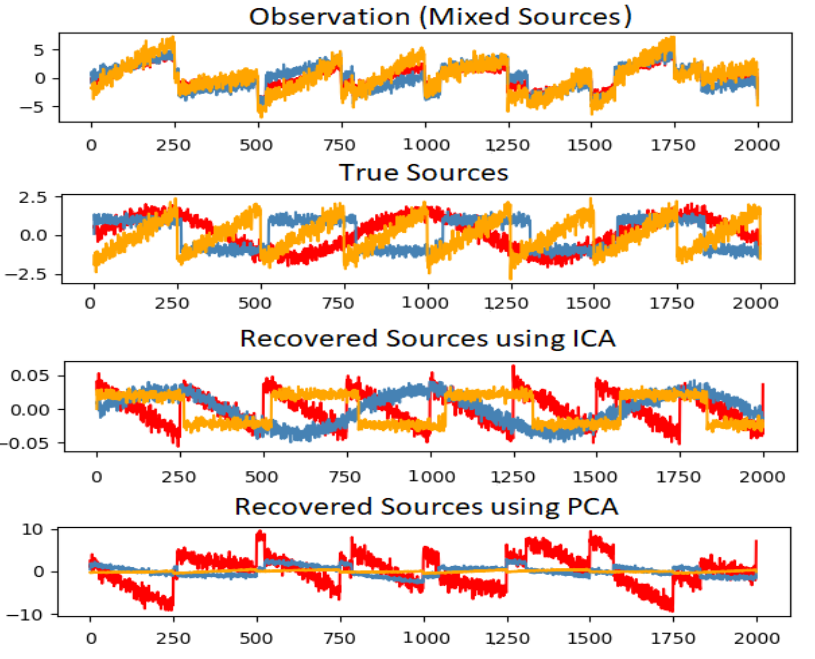
\includegraphics[scale=0.4]{img/06_Linear_Factor/ICA_example.png}
    \end{center}

  \subsection{Slow Feature Analysis} 

    Slow feature analysis also another special case of a linear factor model that uses information from time signals to learn invariant features. It is motivated by a general principle called the \textbf{slowness principle}. The idea is that the important characteristics of scenes change very slowly compared to the individual measurements that make up a description of a scene. For example, in computer vision, individual pixels can change very rapidly. If a zebra moves from left to right across the image, an individual pixel wil rapidly change from black to white. By comparison, the feature indicating whether a zebra is in the image will not change at all, and the feature describing the zebra's position will change slowly. Therefore, we want to regularize our model to learn features that change slowly over time.  

    We can apply the slowness principle to any differentiable model trained with gradient descent. That is, we can add the following term to the loss function: 
    \[\lambda \sum_i d\big( f(\mathbf{x}^{(t+1)}), f(\mathbf{x}^{(t)}) \big)\]
    where $\lambda$ is a hyperparameter determining the strength of the slowness regularization term, $t$ is the time index, $f$ is the feature extractor to be regularized, and $d$ is the distance between $f(\mathbf{x}^{(t)})$ and $f(\mathbf{x}^{(t+1)})$. A common choice for $d$ is the mean squared difference. 

    Essentially, given a set of time-varying input signals $\mathbf{x}^{(t)}$, SFA learns a nonlinear function $f$ that transforms $\mathbf{x}$ into slowly-varying output signals $\mathbf{y}$. Obviously, we can't just take some trivial function like $f = 0$, so we have the following constraints 
    \begin{align*}
        \mathbb{E}_t [ f(\mathbf{x}^{(t)})_i]  & = 0 \\ 
        \mathbb{E}_t [ f(\mathbf{x}^{(t)})_i^2] & = 1 
    \end{align*}
    \begin{center} 
        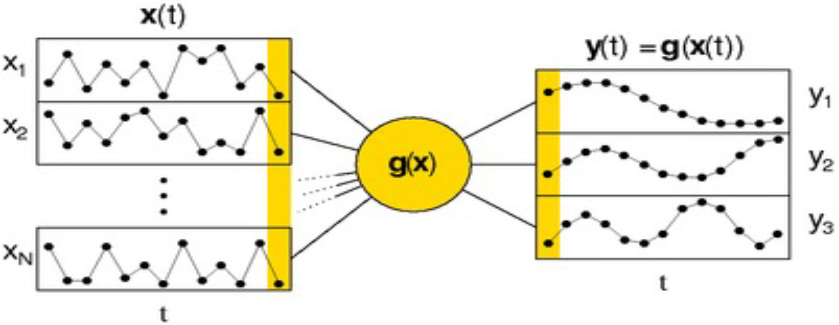
\includegraphics[scale=0.4]{img/06_Linear_Factor/slow_feature.png}
    \end{center}
    We can restrict the nonlinear $f$ to some subspace of functions, and this becomes a standard optimization problem where we solve 
    \[\min_\theta \mathbb{E}_t \big[ \big( f(\mathbf{x}^{(t+1)})_i - f(\mathbf{x}^{(t)})_i \big)^2 \big]\]

  \subsection{Sparse Coding}

    What we want to do in sparse coding is that for each input $\mathbf{x}^{(t)}$, we want to find a latent representation $\mathbf{h}^{(t)}$ s.t. 1) it is sparse (i.e. has many $0$s) and 2) we can reconstruct the original input $\mathbf{x}^{(t)}$ well. We have basically two things to optimize: the latent representations $\mathbf{h}$ and the decoding mechanism, which we can do with a \textbf{dictionary matrix} $\mathbf{D}$. Therefore, we want to perform the joint optimization
    \[\min_{\mathbf{D}} \frac{1}{T} \sum_{t=1}^T \min_{\mathbf{h}^{(t)}} \underbrace{\frac{1}{2} ||\mathbf{x}^{(t)} - \mathbf{D} \mathbf{h}^{(t)}||_2^2}_{\text{reconstruction error}} + \underbrace{\lambda ||\mathbf{h}^{(t)}||_1}_{\text{sparsity penalty}}\]
    To break this term down, let's just assume that we have a fixed dictionary $\mathbf{D}$. Then, we just need to minimize with respect to each $\mathbf{h}^{(t)}$. Now we can add the dictionary parameter back again. 

    Note that the reconstruction, or decoding, of $\mathbf{x}^\prime = \mathbf{D} \mathbf{h}$ is linear and explicit, but if we want to encode $\mathbf{x} \mapsto \mathbf{h}$, we need to substitute the $\mathbf{x}$ into the term above and minimize it w.r.t. $\mathbf{D}$ and $\mathbf{h}$ to solve it. Therefore, this encoder is an implicit and nonlinear function of $\mathbf{x}$. 

    For example, we can reconstruct an image of a seven as a linear combination of a set of images. Note that each of the images of strokes are columns of $\mathbf{W}$ and the coefficients make up the sparse vector $\mathbf{h}$. 
    \begin{center}
        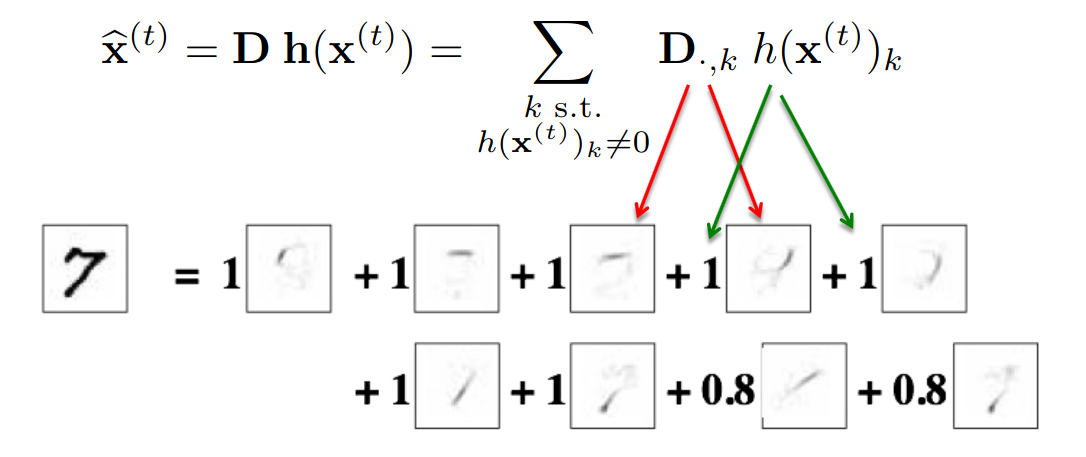
\includegraphics[scale=0.4]{img/06_Linear_Factor/sparse_coding.png}
    \end{center}
    Let's think about how we can optimize the objective function w.r.t. $\mathbf{h}$, keeping $\mathbf{D}$ constant. We can do stochastic gradient descent, which gives us the steps
    \[\nabla_{\mathbf{h}^{(t)}} \mathcal{L}(\mathbf{x}^{(t)}) = \mathbf{D}^T (\mathbf{D} \mathbf{h}^{(t)} - \mathbf{x}^{(t)}) + \lambda \, \mathrm{sign}(\mathbf{h}^{(t)})\]
    but this wouldn't achieve sparsity since it overshoots the $0$ all the time. Therefore, we can clip it, or we can use proximal gradient descent/ISTA to take a step, and shrink the parameters according to the L1 norm. 
    \begin{align*} 
        \mathbf{h}^{(t)} & = \mathbf{h}^{(t)} - \alpha \mathbf{D}^T (\mathbf{D} \mathbf{h}^{(t)} - \mathbf{x}^{(t)}) \\
        \mathbf{h}^{(t)} & = \mathrm{shrink}(\mathbf{h}^{(t)}, \alpha \lambda)
    \end{align*}
        where $\mathrm{shrink}(\mathbf{a}, \mathbf{b}) = [\ldots, \mathrm{sign}(a_i)\, \max(|a_i| - b_i, 0), \ldots]$. This is guaranteed to converge if $1/\alpha$ is bigger than the largest eigenvalue of $\mathbf{D^T} \mathbf{D}$.  

